
\part[Algoritmos sequenciais, condicionais e com repetições]
{Algoritmos sequenciais, condicionais e com repetições}


\chapter[Algoritmos sequenciais]
{Algoritmos sequenciais}



\section{Resumo}

Estrutura sequencial é um conjunto de instruções que serão executadas em sequência. A sequência de cada instrução deve ser seguida apara a realização de uma tarefa.


%\begin{chapreferences}{1.}
%\bibliography{playcb}
%\bibliographystyle{plain}
%\nocite{cbook}
%\nocite{sb6}
%\nocite{glfw}
%\nocite{cppbook}

%\end{chapreferences}

% \begin{chapreferences}{1}

% \bibitem{sb6}
% {\em OpenGL SuperBible}.
% \newblock Pearson Education Inc, 6 edition, 2014.

% \bibitem{glfw}
% Marcus Geelnard and Camilla Berglund.
% \newblock {\em GLFW - Reference guide}, 2010.
% \newblock API version 2.7.

% \bibitem{cbook}
% Brian~W. Kernighan and Dennis~M. Ritchie.
% \newblock {\em The C Programming Language}.
% \newblock 1989.

% \bibitem{cppbook}
% Stanley~B. Lippman, Josés Lajoile, and Barbara Moo.
% \newblock {\em C++ Primer}.
% \newblock 2013.
% \end{chapreferences}

\begin{problems}
\prob
Exiba um plano cartesiano de -100 a 100 com espaçamento de 5 unidades.
\label{ex:cap01_ex1}
\prob
Desenhe um boneco palito que utilize pelo menos uma vez as seguintes geometrias:
\begin{itemize}
\item
Círculo
\item
Elipse
\item
Retângulo
\item
Triângulo
\item
Quadrado
\end{itemize}
\label{ex:cap01_ex2}
\prob
Exiba a estrela de Davi.
\label{ex:cap01_ex3}
\end{problems}


\section{Soluções}

\subsection{\ref{ex:cap01_ex1}Plano Cartesiano}
\begin{figure}[ht]
  \centerline{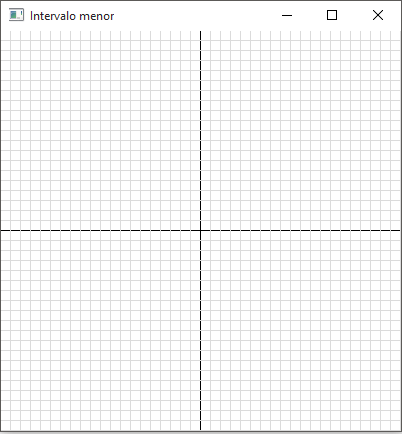
\includegraphics[width=.5\textwidth]{img/cap1_ex1.png}}
  \caption{Plano Cartesiano de -100 à 100}
  \label{fig:cap01_ex1}
\end{figure}

Esta prática se refere a exibir um Plano Cartesiano na tela com espaçamento de 5 em 5 unidades, tanto no eixo x quanto no eixo y. Com ela, o aluno poderá notar a importância da ordem de chamada de funções da playCB e a necessidade das funções \emph{AbreJanela} e \emph{Desenha}, além de verificar, com um exemplo simples, se a playCB foi corretamente bem instalada.
\lstinputlisting[caption=Código fonte de Plano Cartesiano, style=customc, label=lst:cap1_ex1]{src/ex1_PrimeiraJanela.cpp}

\subsection{\ref{ex:cap01_ex2}Boneco Palito}
\begin{figure}[ht]
  \centerline{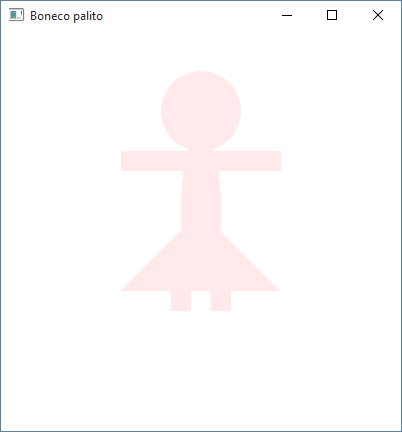
\includegraphics[width=.5\textwidth]{img/cap1_ex3.png}}
  \caption{Boneco Palito}
  \label{fig:cap01_ex2}
\end{figure}
Esta prática se refere a exibir um boneco palito e praticar a grande maioria das geometrias pré-definidas existentes na playCB. Os argumentos de cada função podem ser consultados no Guia de Referência da playCB \footnote{\url{http://pt-br.playcb.wikia.com/wiki/Categoria:Geometrias}}
\lstinputlisting[caption=Código fonte do boneco palito, style=customc, label=lst:cap1_ex2]{src/ex3_boneco.cpp}

\subsection{\ref{ex:cap01_ex3}Estrela de Davi}
\begin{figure}[ht]
  \centerline{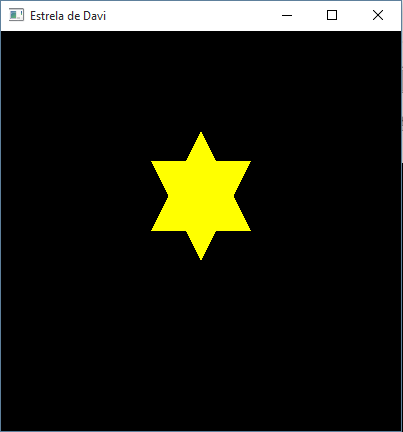
\includegraphics[width=.5\textwidth]{img/cap1_ex2.png}}
  \caption{Estrela de Davi}
  \label{fig:cap01_ex3}
\end{figure}
Esta prática se refere a exibir a estrela de Davi, feita com dois triângulos. Um triângulo foi criado com a função \emph{CriaTriangulo} e o outro com a função \emph{CriaPoligono}. Verificamos nesta prática os argumentos de \emph{CriaTriangulo} (base, altura e ponto esquerdo inferior) e, como não há como ter altura negativa, teve a necessidade de criar um polígono definido pelos três pontos \emph{p1, p2} e \emph{p3} para criar-se um triângulo \emph{de cabeça pra baixo}.
\lstinputlisting[caption=Código fonte da Estrela de Davi, style=customc, label=lst:cap1_ex3]{src/ex2_davi.cpp}


\chapter[Algoritmos condicionais]
{Algoritmos condicionais}



\section{Resumo}

Estrutura condicional expõe que a instrução ou bloco de instrução só seja executada se a condição for verdadeira.


%\begin{chapreferences}{1.}
%\bibliography{playcb}
%\bibliographystyle{plain}
%\nocite{cbook}
%\nocite{sb6}
%\nocite{glfw}
%\nocite{cppbook}

%\end{chapreferences}

% \begin{chapreferences}{1}

% \bibitem{sb6}
% {\em OpenGL SuperBible}.
% \newblock Pearson Education Inc, 6 edition, 2014.

% \bibitem{glfw}
% Marcus Geelnard and Camilla Berglund.
% \newblock {\em GLFW - Reference guide}, 2010.
% \newblock API version 2.7.

% \bibitem{cbook}
% Brian~W. Kernighan and Dennis~M. Ritchie.
% \newblock {\em The C Programming Language}.
% \newblock 1989.

% \bibitem{cppbook}
% Stanley~B. Lippman, Josés Lajoile, and Barbara Moo.
% \newblock {\em C++ Primer}.
% \newblock 2013.
% \end{chapreferences}

\begin{problems}
\prob
Escreva um programa que receba do usuário um valor de ângulo em graus, converta para radianos, exiba uma reta com comprimento de 50 unidades e pinte-a de acordo com as seguintes regras:
\begin{itemize}
\item
Se a reta pertencer ao \emph{primeiro} quadrante, pinte-a de vermelho
\item
Se a reta pertencer ao \emph{segundo} quadrante, pinte-a de verde
\item
Se a reta pertencer ao \emph{terceiro} quadrante, pinte-a de azul
\item
Se a reta pertencer ao \emph{quarto} quadrante, pinte-a de preto
\end{itemize}.
\label{ex:cap01_ex4}
\end{problems}

\section{Soluções}

\subsection{\ref{ex:cap01_ex4}Quadrante de uma reta}
\begin{figure}[ht]
  \centerline{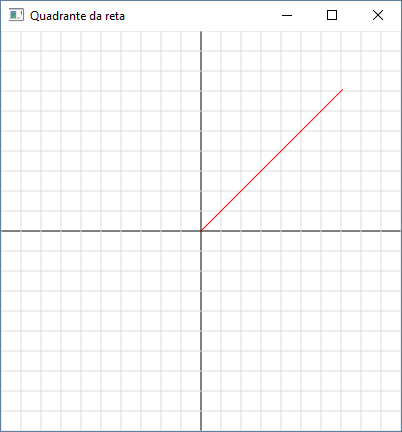
\includegraphics[width=.5\textwidth]{img/cap1_ex4.png}}
  \caption{Determinação do quadrante de uma reta baseado no ângulo de inclinação dela}
  \label{fig:cap01_ex4}
\end{figure}
Esta prática exibe uma reta com cor variada de acordo com qual quadrante ela pertence. A função \emph{Pintar} neste caso se refere a única geometria criada no programa, no caso, a reta.
\lstinputlisting[caption=Código fonte do quadrante da reta, style=customc, label=lst:cap1_ex4]{src/ex4_reta.cpp}


\chapter[Algoritmos com repetição]
{Algoritmos com repetição}



\section{Resumo}

Estruturas de repetição são criadas para que diversas instruções sejam executadas um determinado número de vezes, enquanto a condição se manter verdadeira.


%\begin{chapreferences}{1.}
%\bibliography{playcb}
%\bibliographystyle{plain}
%\nocite{cbook}
%\nocite{sb6}
%\nocite{glfw}
%\nocite{cppbook}

%\end{chapreferences}

% \begin{chapreferences}{1}

% \bibitem{sb6}
% {\em OpenGL SuperBible}.
% \newblock Pearson Education Inc, 6 edition, 2014.

% \bibitem{glfw}
% Marcus Geelnard and Camilla Berglund.
% \newblock {\em GLFW - Reference guide}, 2010.
% \newblock API version 2.7.

% \bibitem{cbook}
% Brian~W. Kernighan and Dennis~M. Ritchie.
% \newblock {\em The C Programming Language}.
% \newblock 1989.

% \bibitem{cppbook}
% Stanley~B. Lippman, Josés Lajoile, and Barbara Moo.
% \newblock {\em C++ Primer}.
% \newblock 2013.
% \end{chapreferences}

\begin{problems}
\prob
Sabendo que a equação hiperbólica pode ser defina por
$$
\begin{matrix}
x	& = &	a \cos(\theta) \\ 
y	& = &	a \sin(\theta)
\end{matrix}.
$$
onde $a$ é a assíntota para y e $\theta$ o ângulo equivalente ao ângulo em coordenadas polares, exiba duas espirais hiberbólicas, onde uma delas está invertida em relação a outra e coloque-as para girar.
\label{ex:cap01_ex5}

\prob
Exiba um carrinho se movendo de $-100$ à $100$.
\label{ex:cap01_ex6}

\prob
Construa um moinho de vento e coloque apenas as hélices para girar.
\label{ex:cap01_ex7}
\end{problems}

\section{Soluções}

\subsection{\ref{ex:cap01_ex5}Galáxia espiral}
\begin{figure}[ht]
  \centerline{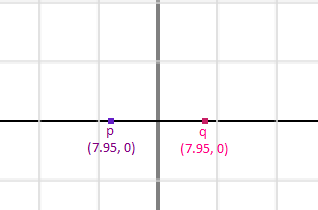
\includegraphics[width=.5\textwidth]{img/cap1_ex6.png}}
  \caption{Duas espirais hiperbólicas girando}
  \label{fig:cap01_ex5}
\end{figure}
Esta prática ilustra como a função \emph{Desenha1Frame} funciona. Na linha 23 até a linha 30, a cada frame são criados dois pontos, um de cada espiral.
\lstinputlisting[caption=Código fonte da galáxia expiral, style=customc, label=lst:cap1_ex5]{src/ex6_galaxy.cpp}

\subsection{\ref{ex:cap01_ex6}Carro andando}
\begin{figure}[ht]
  \centerline{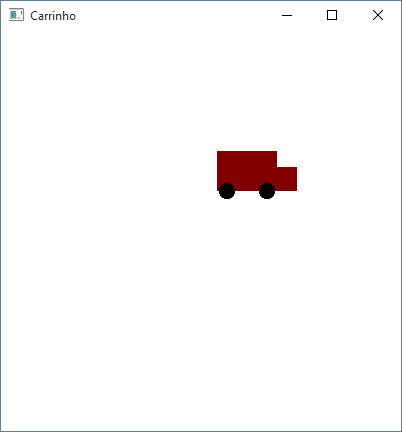
\includegraphics[width=.5\textwidth]{img/cap1_ex5.png}}
  \caption{Carro se movendo da posição -100 até a posição 100}
  \label{fig:cap01_ex6}
\end{figure}
Esta prática exibe um carro construído com dois retângulos e dois círculos, agrupados com a função \emph{CriaGrupo}, movendo-se da posição -100 até a posição 100. Nota-se que todas as geometrias que estão abaixo da função \emph{CriaGrupo} pertencem a um único grupo, o grupo \emph{carro}.
\lstinputlisting[caption=Código fonte do carro andando, style=customc, label=lst:cap1_ex6]{src/ex5_carrinho.cpp}

\subsection{\ref{ex:cap01_ex7}Moinho de vento}
\begin{figure}[ht]
  \centerline{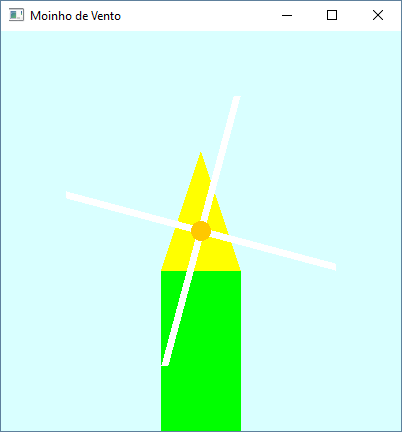
\includegraphics[width=.5\textwidth]{img/cap1_ex7.png}}
  \caption{Moinho de vento}
  \label{fig:cap01_ex7}
\end{figure}
Esta prática exibe um moinho de vento criado com um grupo composto por um triângulo e um retângulo, o grupo \emph{moinho}, e outro grupo composto pelas hélices, o grupo \emph{grupo}. Somente o \emph{grupo} sofre a ação de girar. \footnote{Exemplo criado pelo aluno Pedro Paulo de Pinho Matos, da turma de Computação Básica de 1/2014}
\lstinputlisting[caption=Código fonte do moinho, style=customc, label=lst:cap1_ex7]{src/ex7_moinho.cpp}
